\documentclass[]{article}
\usepackage{graphicx}
\usepackage[spanish]{babel}
\usepackage[a4paper, top=2.5cm, bottom=2.5cm, left=3cm, right=3cm]{geometry}
\usepackage[hidelinks]{hyperref}
\usepackage[T1]{fontenc}
\usepackage{listings}
\usepackage{xcolor}

\definecolor{miverde}{rgb}{0,0.6,0}

% style for listings (código)
\lstdefinestyle{mystyle} {
    stringstyle=\color{miverde},
    breaklines=true,
    breakatwhitespace=false,
    captionpos=b,
    keepspaces=true,
    numbers=none,
    numbersep=5pt,
    showspaces=false,
    showstringspaces=false,
    showtabs=false,
    tabsize=2
}
\lstset{style=mystyle}
\lstset{basicstyle=\ttfamily}

%title
\title{Práctica 1} 

\author{Adrián Ferández Galán, César López Mantecón y Manuel Gómez-Plana Rodríguez}

\begin{document}

\begin{titlepage}
    \centering
   
\includegraphics[width=0.9\textwidth]{uc3m.jpg} 
    {\Huge Universidad Carlos III\\
    
     \Large Arquitectura de Datos\\
     \vspace{0.5cm}
     Curso 2024-25}
    \vspace{2cm}

    {\Huge \textbf{Práctica 1} \par}
    \vspace{0.5cm}
    {\Large Diseño de una Base de Datos No Relacional \par}
    \vspace{8cm}

   \textbf{Ingeniería Informática, Cuarto curso}\\
    \vspace{0.2cm} 
    Adrián Fernández Galán       (NIA: 100472182, e-mail: 100472182@alumnos.uc3m.es)\\
    César López Mantecón         (NIA: 100472092, e-mail: 100472092@alumnos.uc3m.es)\\
    Manuel Gómez-Plana Rodríguez (NIA: 100472092, e-mail: 100472092@alumnos.uc3m.es)
    \vspace{0.5cm}

   
    \textbf{Prof .} Lourdes Moreno López\\
    
    \textbf{Grupo: } 81   
    
\end{titlepage}
\newpage

\renewcommand{\contentsname}{\centering Índice}
\tableofcontents

\newpage

\section{Introducción}
\label{sec:introduccion}
En este documento se recoge el desarrollo de la primera práctica de la asignatura Arquitectura de datos. A continuación, se especifica el diseño de la base de datos a través de un diagrama de clases UML, el diseño de agregados y las estrategias para la validación del esquema.

\section{Diseño conceptual: diagrama de clases UML}
\label{sec:disenno}
En esta sección se describe el primer modelo conceptual teniendo en cuenta tanto la semántica extraída de la descripción de la práctica como de los casos de uso.

Podemos extraer la existencia de 8 entidades importantes en nuestro modelo:
\begin{enumerate}
    \item \textbf{Área:} Representación de cada una de las áreas recreativas. Deben contener información sobre el clima, los \textit{juegos} que contiene, el distrito al que pertenecen, su estdo y su accesibilidad; entre otros.
    \item \textbf{Juego:} Representación de cada uno de los instrumentos en un \textit{área recreativa}. Contiene información sobre el modelo, estado, patrones de desgaste, etc.
    \item \textbf{Clima:} Contiene información meteorológica para una fecha.
    \item \textbf{Historial de intervenciones:} Matiene registro de las \textit{intervenciones} realizadas en un juego.
    \item \textbf{Intervención:} Representa una revisión o intervención sobre un \textit{juego}. Debe contener información sobre la fecha y observaciones realizadas sobre el \textit{juego}.
    \item \textbf{Usuario:} Contiene información sobre un usuario como la información de contacto.
    \item \textbf{Incidencia:} Contiene la información relativa a una incidencia sobre un \textit{juego}. Esto es, naturaleza de la incidencia, lista de usuarios que han reportado la incidencia, estado de la incidencia, empresa encargada de solucionarla, fecha de apertura, fecha de cierre y creador.
    \item \textbf{Encuesta:} Registra información sobre la satisfacción de los \textit{usuarios} para un \textit{juego}.
\end{enumerate}
Con todo lo anterior, hemos realizado el siguiente diseño del sistema.

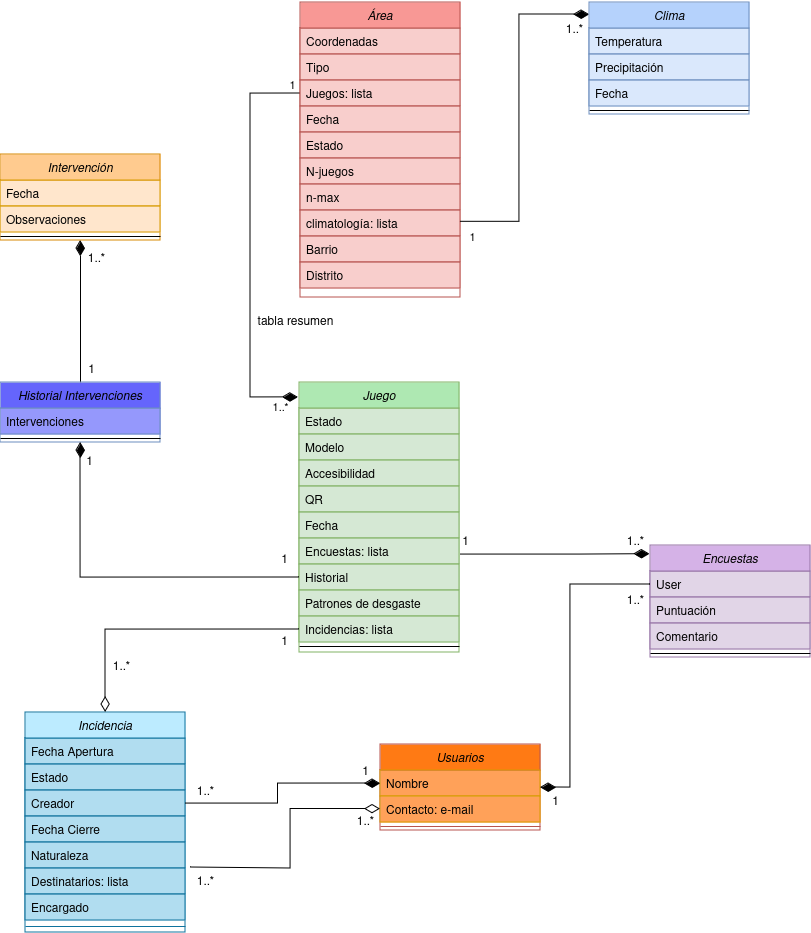
\includegraphics[width=0.9\textwidth]{diagrama_arqui-noaggregados.png}

\subsection{Caso de uso A}
\label{subsec:casoA}
Este caso se centra en proporcionar un listado completo sobre los juegos instalados en diferentes áreas permitiendo una búsqueda por barrio, distrito o área. Por esto se incluyen los campos \textit{distito}, \textit{barrio} en \textit{área}. En el diagrama contiene toda la información necesaria para satisfacer la totalidad de los requistos.

\subsection{Caso de uso B}
\label{subsec:casoB}
Este caso de uso otorga a los usuarios la capacidad de abrir o completar una incidencia en relación a alguno de los juegos de un área recreativa. En el diagrama actual contiene toda la información necesaria para cubrir la totalidad de los requisitos.

\subsection{Caso de uso C}
\label{subsec:casoC}
En este caso se relaciona la información climática con los \textit{juegos} y \textit{áreas}. Por esto se incluyen la entidad \textit{clima} y el campo \textit{patrones de desgaste} en juego. A través de esta información todos los requisitos quedan contemplados en el diagrama.

\subsection{Caso de uso D}
\label{subsec:casoD}
Este caso de uso permite relacionar las incidencias reportadas por los usuarios y las encuestas de satisfacción para mejorar la seguridad, accesibilidad y satisfacción de los ciudadanos. Gracias a las entidades \textit{Incidencia}y \textit{Encuesta} y los campos \textit{encuestas} e \textit{incidencias} en juego recogemos toda la información necesaria para cumplir los 4 requisitos recogidos en este caso de uso.

\subsection{Caso de uso E}
\label{subsec:casoE}
Este caso de uso permite recoger toda la información relativa a las áreas recreativas para la generación de un informe. Gracias a las entidades \textit{historial de intervenciones} y \textit{áreas} el diseño recoge los datos necesarios para generar el informe requerido.

\subsection{Conclusiones sobre el modelo}
\label{subsec:conclusiones-modelo}
Anteriormente hemos visto como el diseño recoge toda la información necesaria para cumplir los 5 casos de uso propuestos en el enunciado. Es por esto que concluímos que se trata de un buen diseño que cumple con las espectativas del sistema.

\newpage
\section{Diseño de agregados}
\label{sec:agregados}
Con el objetivo de poder analizar las capacidades que tendrán los agregados es necesario conoecer las acciones que conllevan los distintos casos de uso.
\begin{itemize}
    \item \textbf{Lectura}: Casos de Uso A y E
    \item \textbf{Escritura}: Casos de Uso B, C y D
\end{itemize}

En el diseño de agregados para el sistema de áreas y sus juegos sea han creado 2 agregados, cada uno optimizado para casos de uso específicos. En estos agregados se ha buscado un equilibrio entre lecturas y escrituras para aquellos agregados enfocados a las inserciones.

Además hemos determinado si las relaciones entre entidades deben de ser embebidas, referencias o tablas resumen. Estas decisiones se fundamentan en la frecuencia de lectura, modificación y crecimiento de los datos.

A continuación se describirán los agregados y las entidates que lo conforman, además de abordar las características de los agregados, como son la raíz y el perímetro.

\subsection{Agregado sobre Áreas y Juegos}
\label{sub_sec:agregado_area_juego}
\begin{itemize}
    \item \textbf{Entidades}: Área, Clima, Historial Intervenciones, Intervención y Juego
    \item \textbf{Raíz}: Área
    \item \textbf{Perímetro}: Este agregado está enfocado en poder consultar la información relevante sobre las áreas y los juegos que lo comprenden y agregar nuevos tiempos climatológicos a las áreas. Cada juego está asociado al área al que pertenece.
    \item \textbf{Casos de Uso optimizados}:
    \begin{itemize}
        \item CU\_A : (Listado detallado de juegos y su estado): Este agregado proporciona consultas rápidas para obtener información sobre los juegos y su estado actual. 
        \item CU\_C : (Impacto del clima en el mantenimiento de juegos): Este agregado permite analizar cómo las condiciones climáticas afectan el desgates de los juegos en las áreas recreativas.
        \item CU\_E : (Informe agrupado por distritos): También es capaz de generar un informe agrupado por distritos que muestre información sobre sus juegos. 
    \end{itemize}
    \item \textbf{Embeber vs Referencias}
    \begin{itemize}
        \item Lecturas frecuentes (CU\_A, CU\_E): Para poder realizar las consultas de estos dos casos de uso se ha optado por embeber las intervenciones en el historial de intervenciones que a la vez está embebidos en sus respectivos juegos.
        \item Inserciones frecuentes (CU\_C): Con el objetivo de que las inserciones no sean costosas se ha decidido embeber el clima en el área, ya que clima será redundante en ninguna otra agregación.
        \item Tabla resumen: Se ha decidido incluir una tabla resumen entre Área y Juego con el objetivo de realizar lecturas rápidas para aquellos atributos estáticos y poder realizar inserciones en juego (dado que juego se encuentra en dos agregados) sin ser costosas.
    \end{itemize}
    \item \textbf{Uso de Índices}
    \begin{itemize}
        \item Para poder realizar búsquedas de todas las áreas de un distrito se ha optado por usar un índice que permita obtener todas las áreas de un distrito, de esta mánera no será necesario realizar una búsqueda exhaustiva
    \end{itemize}
\end{itemize}

\subsection{Agregado sobre Incidencias y Encuestas}
\label{sub_sec:agregado_inserciones_encuestas}
\begin{itemize}
    \item \textbf{Entidades}: Juego, Incidencia, Usuario y Encuestas
    \item \textbf{Raíz}: Juego
    \item \textbf{Perímetro}: Este agregado permite generar informes sobre las incidencias de los juegos y el grado de satisfacción de los usuarios sobre los diferentes juegos.
    \item \textbf{Casos de Uso optimizados}:
    \begin{itemize}
        \item CU\_B : (Proceso de mantenimiento del mobiliario urbano): Este agregado proporciona la capacidad generar incidentes en los juegos.
        \item CU\_D : (Mejora la toma de decisiones con incidentes de seguridad y satisfacción): Este agregado permite almacenar nuevas encuestas sobre los juegos y generar informes con las correlaciones entre las incidencias y las encuestas de un mismo juego. 
    \end{itemize}
    \item \textbf{Embeber vs Referencias}
    \begin{itemize}
        \item Lecturas frecuentes (CU\_B y CU\_D): Para realizar los diferentes informes de ambos casos de uso se necesita consultar las incidencias y las encuestas almacenadas. Las encuestas se implementarán de forma embebida para reducir el coste de lectura. Las incidencias se implementarán como referencias ya que consideramos que, aunque quede fuera de los casos de uso, las incidencias se actualizarán con frecuencia lo que nos permitirá reducir el coste de las actualizaciones. 
        \item Inserciones frecuentes (CU\_B y CU\_D): Dadas las características mencionadas con anterioridad tanto las encuestas como las incidencias tendrán un coste reducido, dado que las incidencias se implementan como referencias y las encuestas de forma embebida pero no existirán otras copias. Estas inserciones en juego no afectarán al anterior agregado ya que se implementó como una tabla resumen donde los datos que cambian se obtendrán por referencia y los datos no cambiantes irán dentro del resumen
    \end{itemize}
\end{itemize}

[Imagen con agregados]

\subsection{JSONs de ejemplos}
\label{sub_sec:json_ejemplos}
Para poder visualizar de una manera más práctica los agregados, a continuación se ejemplifica en formato JSON cada uno de los agregados. 
\begin{itemize}
    \item \textbf{Agregado sobre áreas y juegos}
\end{itemize}
\begin{lstlisting}[caption=Ejemplo de JSON para Agregado sobre Áreas y Juegos, language=C]
{
    "Coordenadas": "36 30 10.0 N 6 16 30.0 W",
    "Tipo": "Parque infantil",
    "Fecha": "2024/09/26 10:23:49",
    "Estado": "Operativa",
    "N-Juegos": 2,
    "N-Max": 50,
    "Barrio": "Barrio de Puntuales",
    "Distrito": "Cadiz",
    "Climatologia": [
        {
            "Fecha": "2024/09/26 23:59:59",
            "Temperatura": 23,
            "Precipitacion": 0
        },
        {
            "Fecha": "2024/09/27 23:59:59",
            "Temperatura": 27,
            "Precipitacion": 0
        }
    ],
    "Resumen Juego": [
        {
            "_id": 1,
            "Modelo": "Columpio",
            "Accesibilidad": [
                "Silla de ruedas",
                "Muletas"
            ],
            "QR": imagen,
            "Fecha": "2024/09/26 10:00:00"
        },
        {
            "_id": 2,
            "Modelo": "Balancin",
            "Accesibilidad": [
                "Muletas"
            ],
            "QR": imagen,
            "Fecha": "2024/09/26 10:15:00"
        }
    ]
}
\end{lstlisting}

\begin{itemize}
    \item \textbf{Agregado sobre áreas y juegos}
\end{itemize}
\begin{lstlisting}[caption=Ejemplo de JSON para Agregado sobre Indicencias y Encuestas, language=C]
{
    "Estado": "Disponible",
    "Modelo": "Columpio",
    "Accesibilidad": [
        "Silla de ruedas",
        "Muletas"
    ],
    "QR": imagen,
    "Fecha": "2024/09/26 10:00:00""Accesibilidad"
    "Patrones de desgaste": [
        "Lluvia",
        "Fuego"
    ],
    "Encuestas": [
        {
            "Puntuacion": 4.6,
            "Comentario": "Buena localizacion con un un ambiente tranquilo",
            "User": {
                "Nombre": "Ernesto",
                "Contacto": "ernesto_2010@gmail.com"
                }
        },
        {
            "Puntuacion": 5.0,
            "Comentario": "Muy buena atraccion para mis hijos, 100% recomendado",
            "User": {
                "Nombre": "Mari Pili",
                "Contacto": "lapili_mari@gmail.com"
            }
        }
    ]
    "Incidencias": [
        {
            "Fecha Apertura": "2024/09/26 16:00:30",
            "Estado": "Cerrada",
            "Creador": {
                "Nombre": "Pablo",
                "Contacto": "_pablo_@gmail.com"
            },
            "Fecha Cierre": "2024/09/26 17:31:48",
            "Naturaleza": "Fallo de estructura",
            "Destinatarios": [
                {
                    "Nombre": "Pablo",
                    "Contacto": "_pablo_@gmail.com"
                },
                {
                    "Nombre": "Ernesto",
                    "Contacto": "ernesto_2010@gmail.com"
                }
            ],
            "Encargdo": "Natalia Garcia Lopez"
        }
    ]
}
\end{lstlisting}

\newpage
\section{Validación del esquema}
\label{sec:esquema}
Para mantener la integridad de los datos, MongoDB ofrece el uso de estrategias como el uso de referencias en vez de embeber los datos. Sin embargo, para aquellos datos que hemos decidido embeber, debemos redactar una serie de reglas para mantener la consistencia de nuestro esquema. Estas reglas son:
\begin{itemize}
    \item \textbf{Coordenadas de \textit{Área}}: Las coordenadas de las áreas serán un string que contenga en grados, minutos, segundos y dirección la latitud y longitud del área. Además, los grados deben ser números enteros no negativos menores de 91, los minutos y segundos deben ser números flotatntes no negativos menores o iguales a 60 y la dirección tendrán los valores ``N'' o ``S'' para la latitud y ``E'' o ``W'' para la longitud.
    \item \textbf{Tipo de \textit{Área}}: El tipo de un área solo puede guardar los valores: ``Parque infantil'', ``Zona deportiva'' y ``Espacio para mayores''.
    \item \textbf{Estado Operativo \textit{Área}}: El estado operativo de las áreas sólo podrán guardar los valores ``Operativa'', ``En Mantenimiento'' y ``Fuera de servicio''.
    \item \textbf{Número de Juegos \textit{Área}}: El número de juegos instalados en un área debe ser un entero no negativo y siempre menor o igual al número máximo de juegos de un área.
    \item \textbf{Número Máximo de Juegos \textit{Área}}: El número máximo de juegos de un área debe ser un enterno no negativo.
    \item \textbf{Temperatura \textit{Clima}}: La temperatura de \textit{Clima} es un float y se medirá en grados Celsius.
    \item \textbf{Precipitación \textit{Clima}}: La precipitación de \textit{Clima} es un float y se medirá en litros por metro cuadrado.
    \item \textbf{Estado Operativo \textit{Juego}}: El estado operativo de los juegos sólo podrá guardar dos valores ``Disponible'' o ``No Disponible''.
    \item \textbf{QR \textit{Juego}}: El QR de los juegos debe de ser una imagen.
    \item \textbf{Accesibilidad \textit{Juego}}: La accesibilidad de un juego debe ser un texto que indique las personas con alguna deficiencia física que puedan acceder al juego.
    \item \textbf{Estado \textit{Incidencia}}: El estado operativo de los juegos sólo podrá guardar dos valores ``Abierta'' o ``Cerrada''.
    \item \textbf{Fechas \textit{Incidencia}}: La fecha de apertura debe ser anterior a la fecha de cierre si el estado es ``Cerrada''.
    \item \textbf{Naturaleza \textit{Indicencia}}: Se debe comprobar que no haya una incidencia con la misma naturaleza asociada al mismo objeto antes de introducirla.
    \item \textbf{e-mail de \textit{Usuario}}: El e-mail de los usuarios debe tener un formato válido para poder gestionar el contacto al resolver las incidencias.
    \item \textbf{Fechas}: Las fechas de todas las entidades deben seguir el formato: ``yyyy/mm/dd hh:MM:ss''.
    \item \textbf{Decimal}: Los números flotantes se determinan con un ``.''.
\end{itemize}

\end{document}
